% This sample document was created by P.J. Healy (healy.52@osu.edu) for educational purposes. You may use this as a template for your own documents as you wish.

% Lines that start with a percent sign are just comments - they won't be processed or show up in the final output. If you actually want a percent sign to show up, use \% instead, like ``I got 100\%!''

% \documentclass says what type of document we're making and gives some basic options (options appear in square brackets. Here, our document is like an article (as opposed to a book, report, PhD thesis, etc.), we want 11-point font, and equation numbers on the left (leqno).
\documentclass[11pt,leqno]{article}

% These are the following packages we want LaTeX to load, since we might use them. I group them by similarity.
\usepackage{amsfonts,amsmath,amssymb,amsthm}
\usepackage{color,graphicx}
\usepackage{fullpage,setspace}
\usepackage[colorlinks=true,urlcolor=darkgray,bookmarks=false]{hyperref}

% First we tell LaTeX that we want to create a numbered "theorem-like" environment whose label is "Theorem X" and whose numbering will be handled by an internal counter named "theorem".
\newtheorem{theorem}{Theorem}

% The 'length variable' \parindent says how far to indent each paragraph. I want to set that length variable to zero:
\setlength{\parindent}{0mm}

% At OSU, you might use scarlet and gray colors for things, so here they are. Note: this requires the color package to be loaded. If you don't use this (and I don't below), you might as well comment it out or delete it.
\definecolor{scarlet}{cmyk}{0,1.00,0.65,0.15}
\definecolor{gray}{cmyk}{0.06,0,0,0.34}

\begin{document}


% First, move up from the normal starting point on the page by 20 millimeters so the table appears in the top margins
\vspace*{-20mm}

% Here's the actual table. We start with a `tabular' environment with 3 columns. The column alignments are left, center, and right, respectively, so the command option is {lcr}. Within the table, columns are delimited by & and rows by \\
% Note that LaTeX ignore consecutive spaces, including tabs, so you can use tabs to make your table look reasonable here.
\begin{tabular*}{\textwidth}{@{\extracolsep{\fill}}lcr}
Econ 8714     & \hfill    &         Professor: P.J. Healy          \\
Microeconomic Theory 2B  &           &   TA: Han Wang    
\end{tabular*}

% Finally, let's put a big `title' in the center of the page, after we `skip' down a bit of space.
\bigskip
\begin{center}
{\Large 03/24/2023 Recitation \#3 Handout}
\end{center}

% Skip some more space and then start working
\bigskip

\textbf{1. Environment}


A mechanism design environment $\mathcal{E}=\left\{N,\left\{\Theta_i\right\}_{i \in N}, p, X,\left\{u_i\right\}_{i \in N}\right\}$
\begin{itemize}
    \item $N=\{1,2, \cdots, n\}$ \quad set of agents
    \item $\Theta_{i}$  \quad  set of agent $i$'s types (Write $\Theta=\underset{i\in N}{\Pi}\Theta_{i}$)
    \item $p \in \Delta(\Theta)$ \quad common prior distribution
    \item $X$ \quad set of outcomes (or social alternatives)
    \item $u_{i}: X \times \Theta \rightarrow \mathbb{R}$ \quad agent $i$'s utility function
\end{itemize}
\textbf{Notes:} (1) $\mathcal{E}$ has \emph{independent types}, if $p$ is a product distribution; (2) $\mathcal{E}$ has \emph{private values}, if we can write $u_{i}(x,\theta)=u_{i}(x,\theta_{i})$. 

\textbf{2. Social Choice Function/Correspondence}

\begin{itemize}
\item A social choice function (SCF)
$f: \theta \rightarrow x$ assigns each type profile $\theta$ an outcome $x$.
\item A social choice correspondence (SCC) $F: \Theta \rightrightarrows X$ assigns each type profile $\theta$ a set of outcomes.
\end{itemize}



\textbf{3. Mechanisms}
A mechanism $\Gamma=\left\{ \left\{S_i\right\}_{i \in N},  g\right\}$
\begin{itemize}
    \item $S_{i}$ \quad set of agent $i$'s actions (Write $S=\underset{i\in N}{\Pi}S_{i}$)
    \item $g:S\to X$ \quad outcome function
\end{itemize}

\textbf{Notes:} $\Gamma$ is a direct mechanism if $S_{i}=\Theta_{i}$, $\forall i\in N$.

\begin{figure}[h]
    \centering
    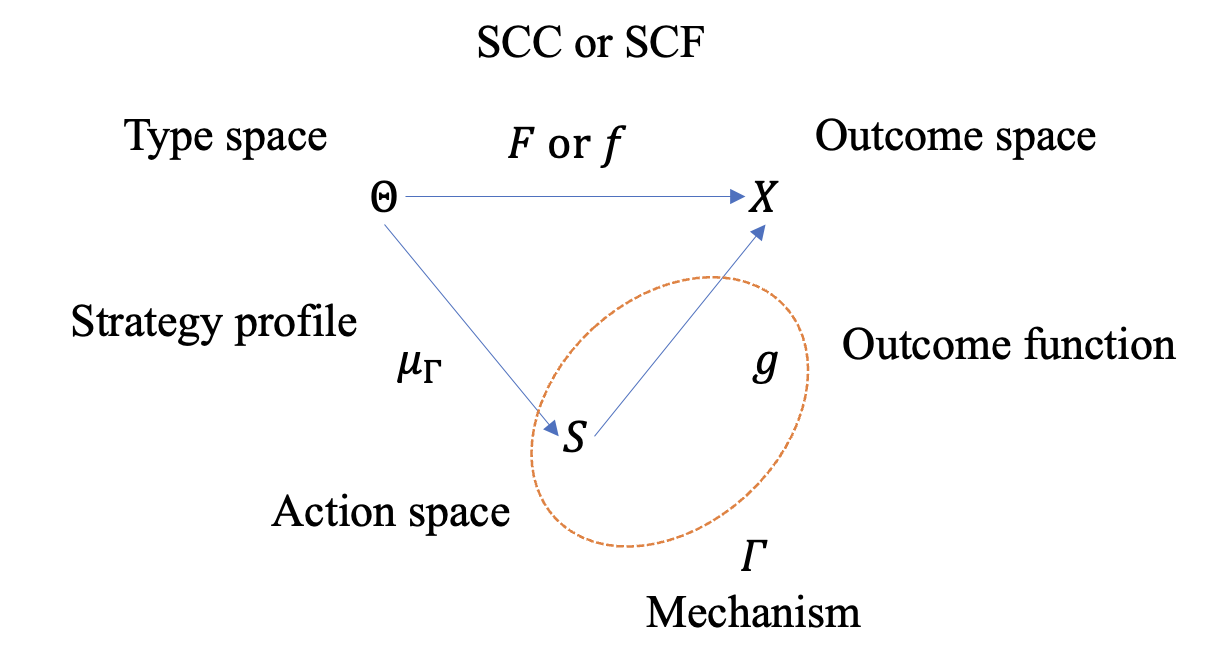
\includegraphics[width=0.5\textwidth]{figure 1.png}
    \caption{The Mount-Reiter Diagram}
    \label{fig:1}
\end{figure}

$\mathcal{E}$ and $\Gamma$ defines a Bayesian game $\mathcal{G}=\left\{N,\left\{S_i\right\}_{i \in N}, \left\{\Theta_i\right\}_{i \in N}, \left\{p_i\right\}_{i \in N}, \left\{v_i\right\}_{i \in N}\right\}$, where agents'  first-order beliefs $p_{i}$ are derived from $p$\footnote{Many applications of Bayesian games employ the common prior assumption---the assumption that the players' first-order beliefs $p_{i}:\Theta_{i}\to \Delta(\Theta_{-i})$ are conditional probabilities generated from some $p$. } and the utility functions are defined by $v_{i}(s,\theta)=u_{i}(g(s),\theta)$.

\newpage

\textbf{4. Implementation}

We need to impose some assumption on $\mu_{\Gamma}$, i.e., to specify the equilibrium concept we are using: dominant strategies, NE, BNE, rationalizability... 

\begin{figure}[h]
    \centering
    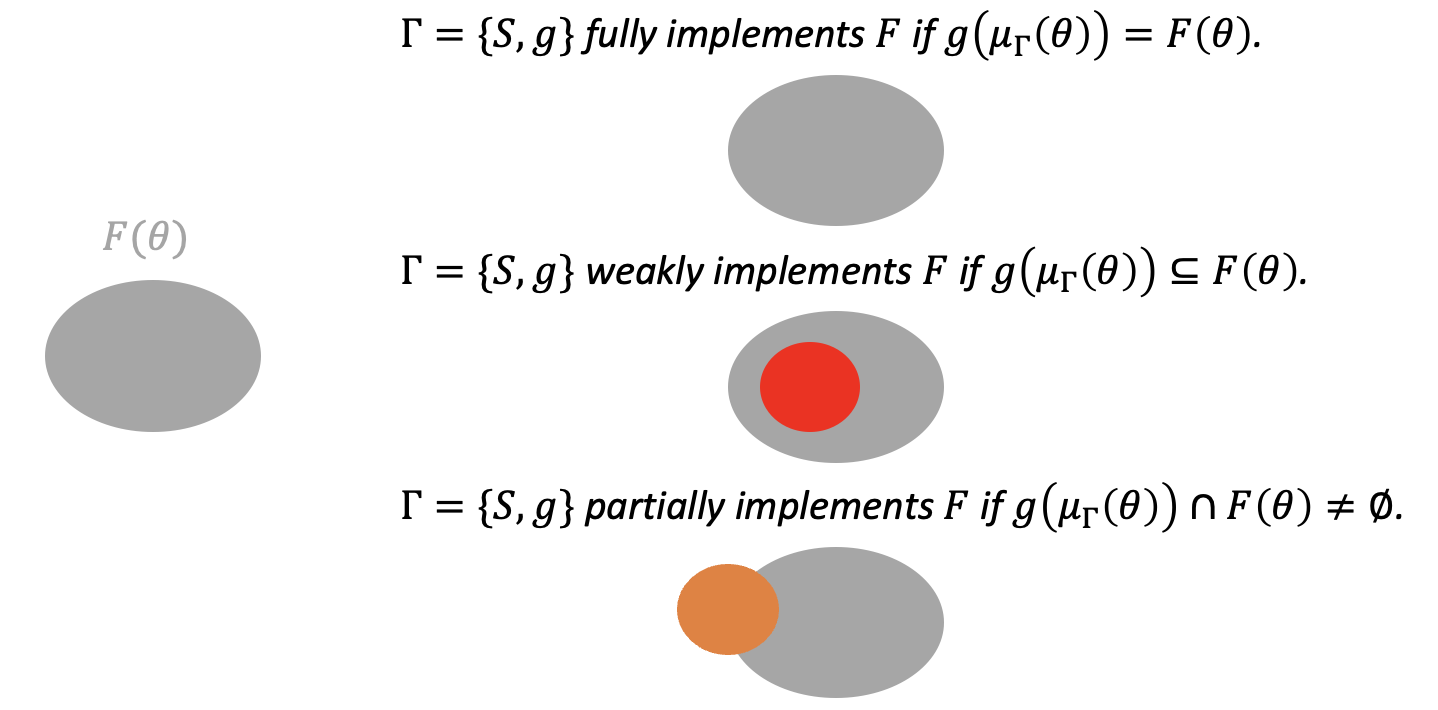
\includegraphics[width=0.5\textwidth]{figure 2.png}
    \caption{Implementation}
    \label{fig:2}
\end{figure}

Our goal is to find a mechanism that implements $F$. It might not be an easy task, since the set of all possible mechanisms is very large.

\textbf{5. Revelation Principle}

We will show that one can focus on mechanisms of a particular simple kind.

To fix ideas, let's consider implementing a social choice function $f$. 

\begin{figure}[h]
    \centering
    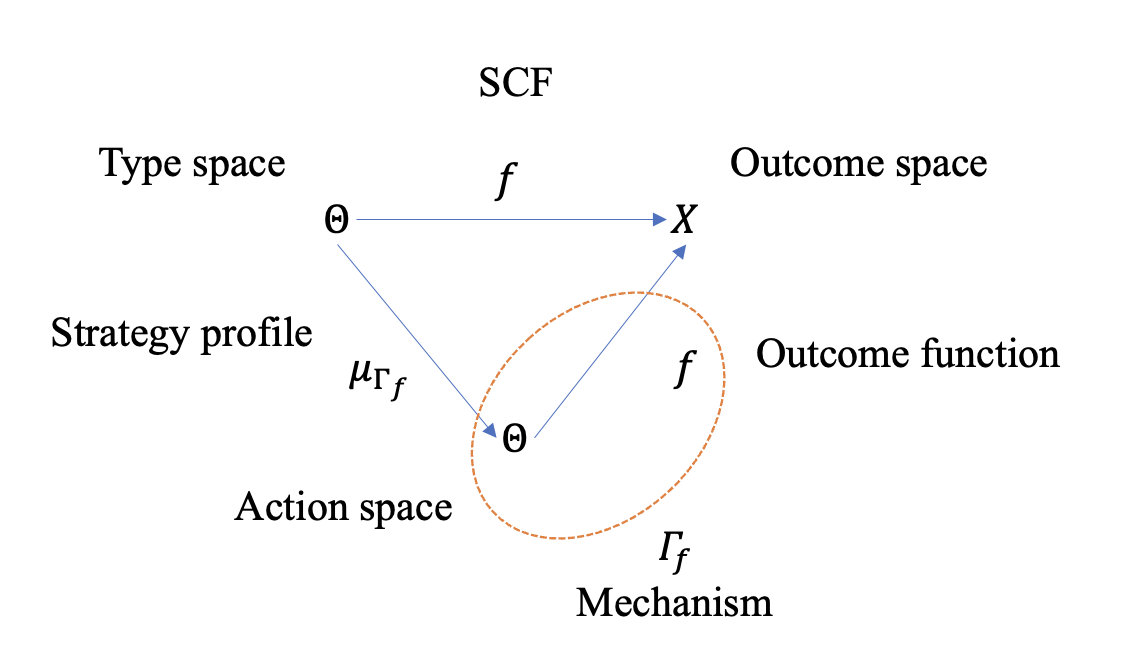
\includegraphics[width=0.5\textwidth]{figure 3.png}
    \caption{$\Gamma_{f}$}
    \label{fig:3}
\end{figure}

\begin{itemize}
    \item $\Gamma_{f}$ is an equivalent direct mechanism for SCF $f$.
    \item $F$ is incentive-compatible (IC) under equilibrium concept $\mu$, if $\forall \theta\in \Theta$, $\theta\in \mu_{\Gamma_{f}}(\theta)$.
\end{itemize}


\begin{theorem}
If there is a $\Gamma=\left\{\left\{S_{i}\right\}_{i\in N}, g\right\}$ that implements $f$ in dominant strategies, then the direct mechanism $\Gamma_{f}=\left\{\left\{\Theta_{i}\right\}_{i\in N}, f\right\}$ truthfully implements $f$ in dominant strategies. Thus, a social choice function is dominant strategy implementable by some mechanism if and only if it is dominant strategy incentive-compatible!
\end{theorem}
\begin{proof}[Sketch of the Proof]
    Simply use $g(\mu_{\Gamma (1)}(\theta_{1}), \mu_{\Gamma (2)}(\theta_{2}),..., \mu_{\Gamma (n)}(\theta_{n}))=f(\theta_{1},...,\theta_{n}), \quad \forall \theta$. 
\end{proof}


\end{document} 